\documentclass[]{beamer}

\newcommand\candidatename{Carrez Valentin}
\newcommand\candidatenumber{31593}

\newcommand\iconwidth{2em}
\newcommand\arrowwidth{0.8mm}

% French language support (e.g. date format)
\usepackage[french]{babel}
\usepackage[T1]{fontenc}
\usepackage{lmodern} % for missing fonts (e.g. italic in titles)

\usetheme[subsectionpage=progressbar]{metropolis}

\title{Résolution de niveaux du Sokoban}
\author{\candidatename}
\date{Candidat n°\candidatenumber}
\def\titlepage{%
  \usebeamertemplate{title page}% <--- avoid overfull vbox on titlepage (see https://tex.stackexchange.com/a/444420)
}

\makeatletter
    \setlength{\metropolis@titleseparator@linewidth}{3pt}
    \setlength{\metropolis@progressonsectionpage@linewidth}{3pt}
    \setlength{\metropolis@progressinheadfoot@linewidth}{3pt}
\makeatother

\setbeamertemplate{footline}[page number] % page numbers <current page> / <total page count>

\usepackage{subcaption} % rules

\usepackage{stmaryrd}
\usepackage{algorithm}
% \captionsetup[algorithm]{labelformat=empty}
\usepackage{algpseudocode}

% Url formatting
\usepackage{href-ul}

\usepackage{multirow} % table with colspan and rowspan

\usepackage{forest} % trees

\usepackage{pgfplots} % graphs

\usepackage{tikz}
\usetikzlibrary{babel}
\usetikzlibrary{arrows, shapes, positioning, shadows, trees, calc, fit, backgrounds}
\usetikzlibrary{overlay-beamer-styles} % 'visible on' option for nodes
\usetikzlibrary{arrows.meta, calc, quotes, tikzmark}
\usetikzlibrary{shapes.multipart, chains, scopes, matrix} % greedy heuristic
% to enable ! in tikz
\tikzset{
    handle active characters in code=false, % (inutile, c’est par défaut)
    handle active characters in nodes, % true/false ne change rien
}

\usepackage{graphics}
    \graphicspath{{../assets/}} % filepath of images (used in \includegraphics{})
\usepackage{subcaption}

% zobrist hashing
\usepackage{blkarray}
\newcommand{\xor}{\, \text{\textbf{XOR}} \,}

\usepackage{stmaryrd} % integer brackets

\usepackage{adjustbox}

\usepackage{xcolor}

\usepackage{copyrightbox}
\makeatletter
\renewcommand{\CRB@setcopyrightfont}{\fontsize{5}{5}\selectfont\color{darkgray}}
\renewcommand{\CRB@setcopyrightparagraphstyle}{\raggedleft}
\makeatother

\pgfplotsset{compat=1.18}
% stats
\definecolor{RED}    {RGB}{220,  57,  18}
\definecolor{GREEN}  {RGB}{16,  150,  24}
\definecolor{BLUE}   {RGB}{48,   96, 193}
\definecolor{ORANGE} {RGB}{255, 153,   0}
\definecolor{MAGENTA}{RGB}{200,  54, 166}
\pgfplotscreateplotcyclelist{mylist}{
    {RED,     line width=1.5, rounded corners=1pt},
    {GREEN,   line width=1.5, rounded corners=1pt},
    {BLUE,    line width=1.5, rounded corners=1pt},
    {ORANGE,  line width=1.5, rounded corners=1pt},
    {MAGENTA, line width=1.5, rounded corners=1pt}% <-- don't add a comma here
}
\usepackage[absolute, overlay]{textpos}
\pgfkeys{/pgf/number format/.cd,
    set thousands separator={\ }}

\definecolor{GRAY250}{RGB}{250, 250, 250}

% Graphiques des résultats intermédiaires

\newenvironment{interstatenv}[2]{%
    \centering
    \footnotesize Niveaux résolus dans \textit{XSokoban} : \textbf{#1 / 90 (+ #2)}

    \footnotesize Niveau 24 du pack \textit{Boxxle} :


    \begin{columns}
        \begin{column}{\dimexpr0.5\paperwidth-10pt}
            \begin{tikzpicture}[scale=0.8]
                \begin{axis}[
                        xtick={0,1,2,3,4,5,6,7,8},
                        xticklabels={Rien, Dead tiles, Tunnels, Salles, Freeze deadlocks, PI-Corral pruning, A*, fess0},
                        xticklabel style={
                            anchor=base,
                            yshift=-1.5\baselineskip,
                            rotate=25,
                            font=\tiny
                        },
                        nodes near coords,
                        nodes near coords style={draw=black, fill=GRAY250, text=RED, outer sep=0, inner sep=0.08cm, yshift=0.15cm, line width=0.2},
                        nodes near coords align={above},
                        axis x line=bottom,
                        axis y line=left,
                        grid=both,
                        ylabel={Nombre d'états explorés},
                        ymode=log,
                        ymin=1000,
                        line width=1.5
                    ]
}{%
                \end{axis}
            \end{tikzpicture}
        \end{column}
        \hfill
        \begin{column}{\dimexpr0.35\paperwidth-10pt}
            \centering
            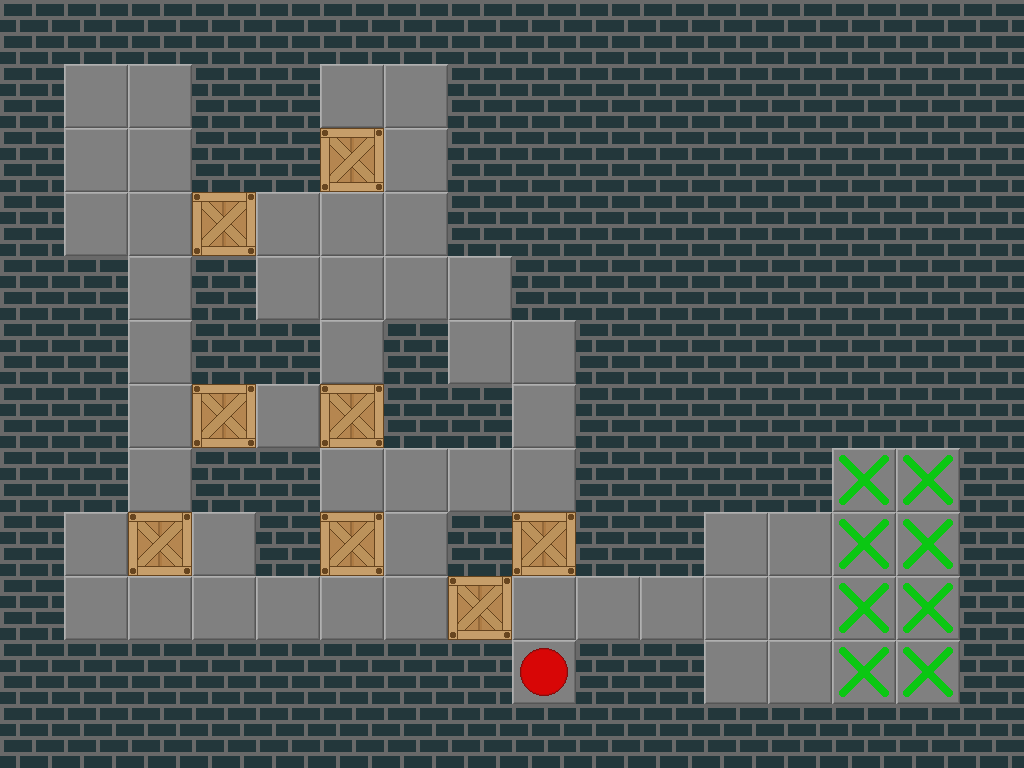
\includegraphics[width=\textwidth]{Boxxle_1_24.png}
        \end{column}
    \end{columns}
}

\newenvironment{interstateframe}{%
    \begin{frame}{Résultats intermédiaires}
        \centering
}{%
    \end{frame}
}

\newcommand\interstatplot[1]{%
    \addplot+ [sharp plot, RED, mark options={fill=RED}, point meta=explicit symbolic, restrict x to domain=0:#1] table[meta=label] {content/inter_stats_data.txt}
}

% Légende en bas de page

\newcommand\BottomLeftText[1]{%
    \begin{textblock*}{\paperwidth}(.5em, 0.99\textheight)
        \raggedright \tiny \textit{#1} \vspace{.5em}
    \end{textblock*}
}